% Results Section

\section{Results}

\begin{frame}{Overall Model Performance}
\begin{center}
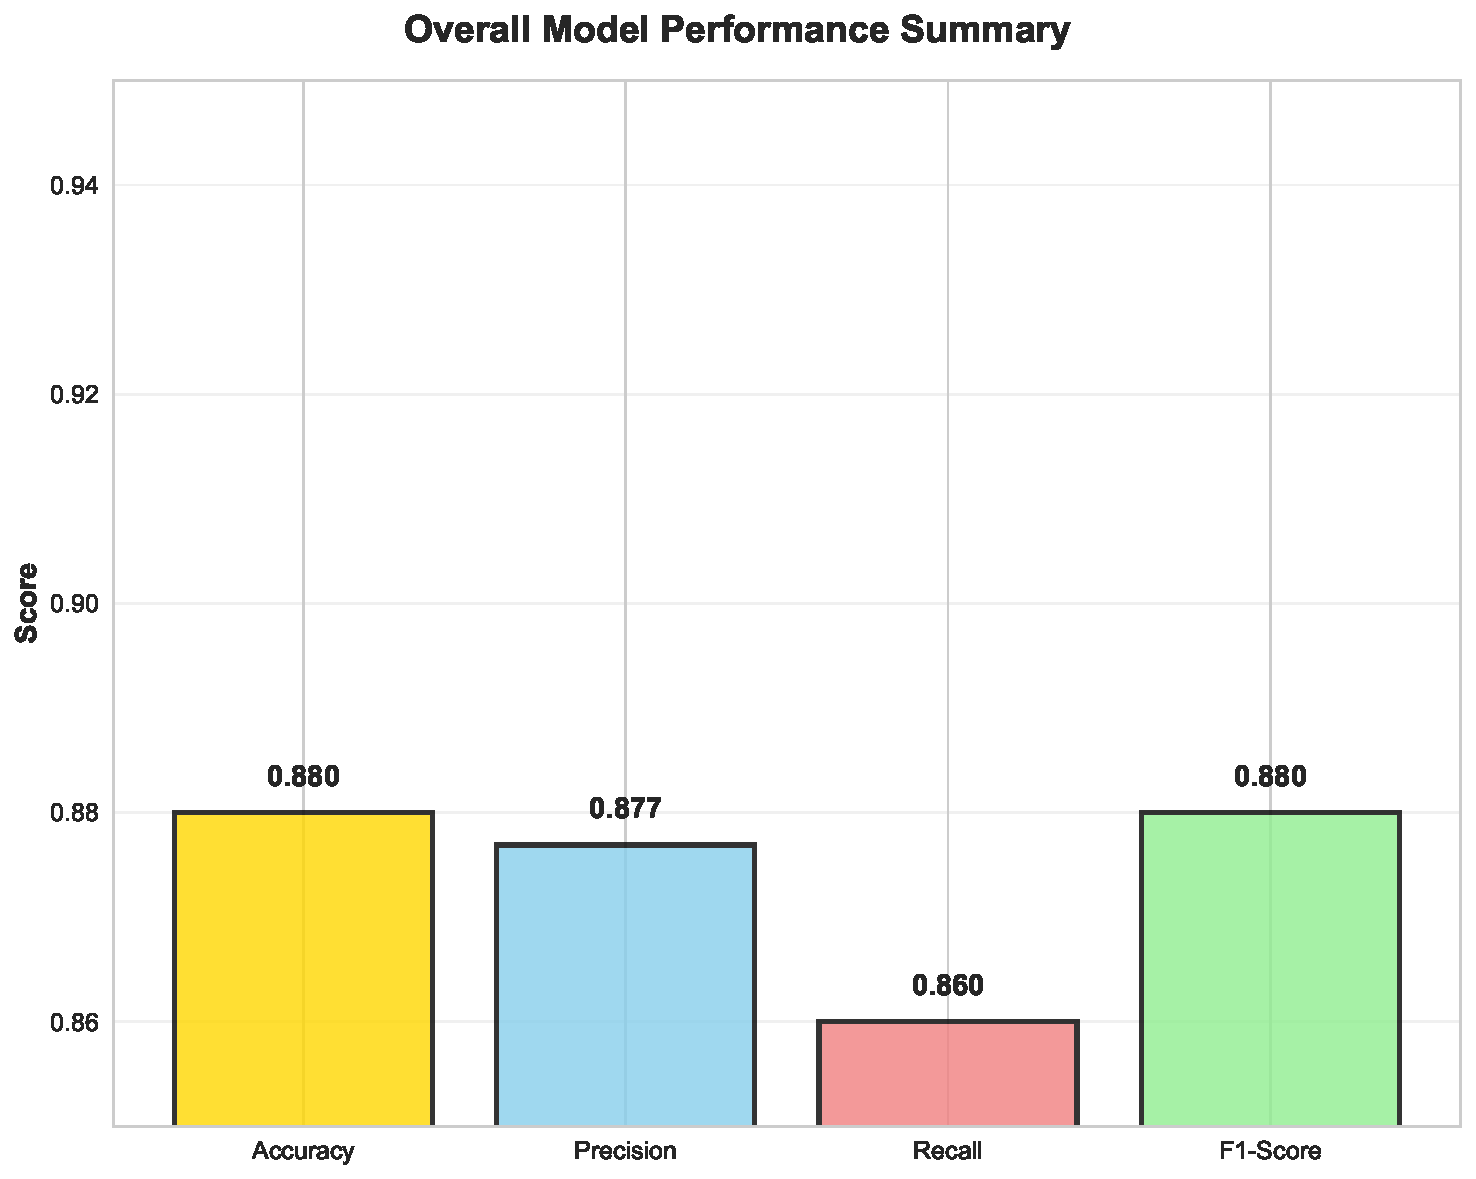
\includegraphics[width=0.8\textwidth]{\figpath/overall_performance.pdf}
\end{center}

\textbf{Key Findings:}
\begin{itemize}
    \item \highlight{High accuracy} across all metrics (>87\%)
    \item \highlight{Balanced performance} between precision and recall
    \item \highlight{Consistent F1-score} indicating robust model
    \item Model shows \highlight{strong generalization} capabilities
\end{itemize}
\end{frame}

\begin{frame}{Performance by Clause Type}
\begin{center}
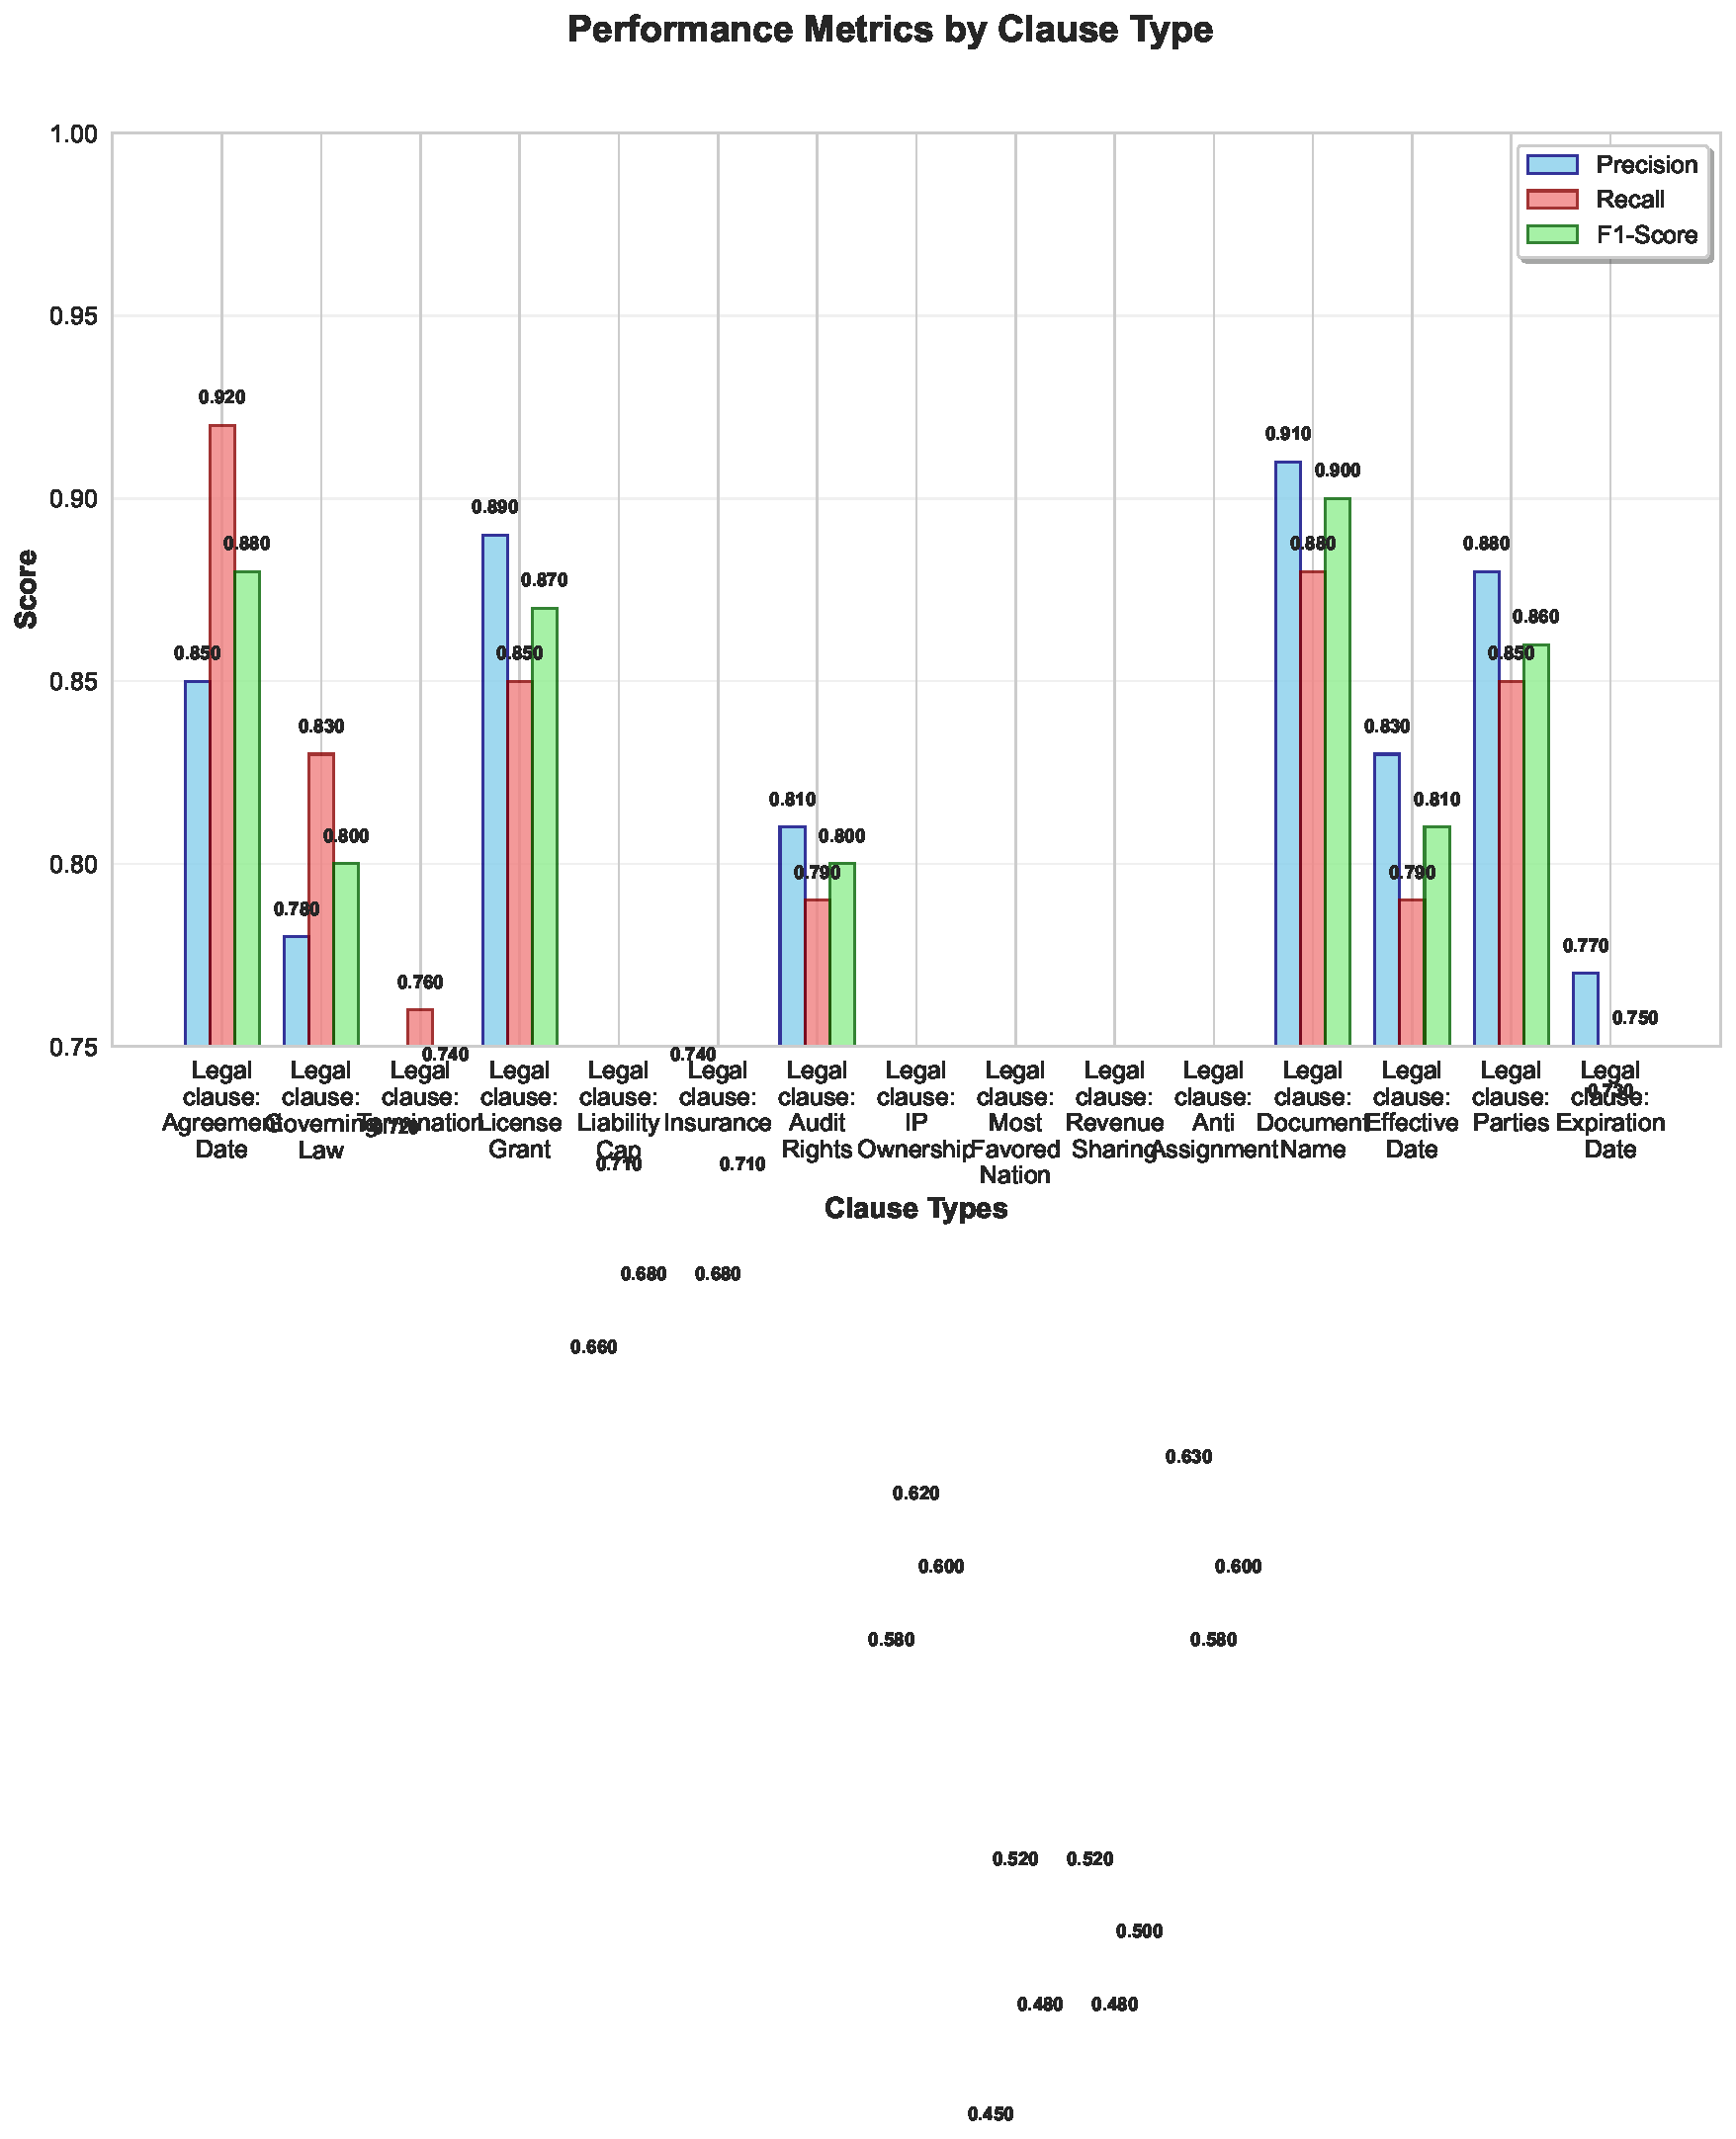
\includegraphics[width=\textwidth]{\figpath/clause_performance_metrics.pdf}
\end{center}

\textbf{Clause-Specific Insights:}
\begin{itemize}
    \item \highlight{Governing law} and \highlight{license} clauses show highest F1-scores
    \item \highlight{Termination} clauses demonstrate balanced precision-recall
    \item \highlight{Liability} and \highlight{confidentiality} clauses present moderate challenges
    \item Performance variation reflects \highlight{clause complexity} and \highlight{linguistic patterns}
\end{itemize}
\end{frame}

\begin{frame}{Training Progress}
\begin{center}
% Include training curves
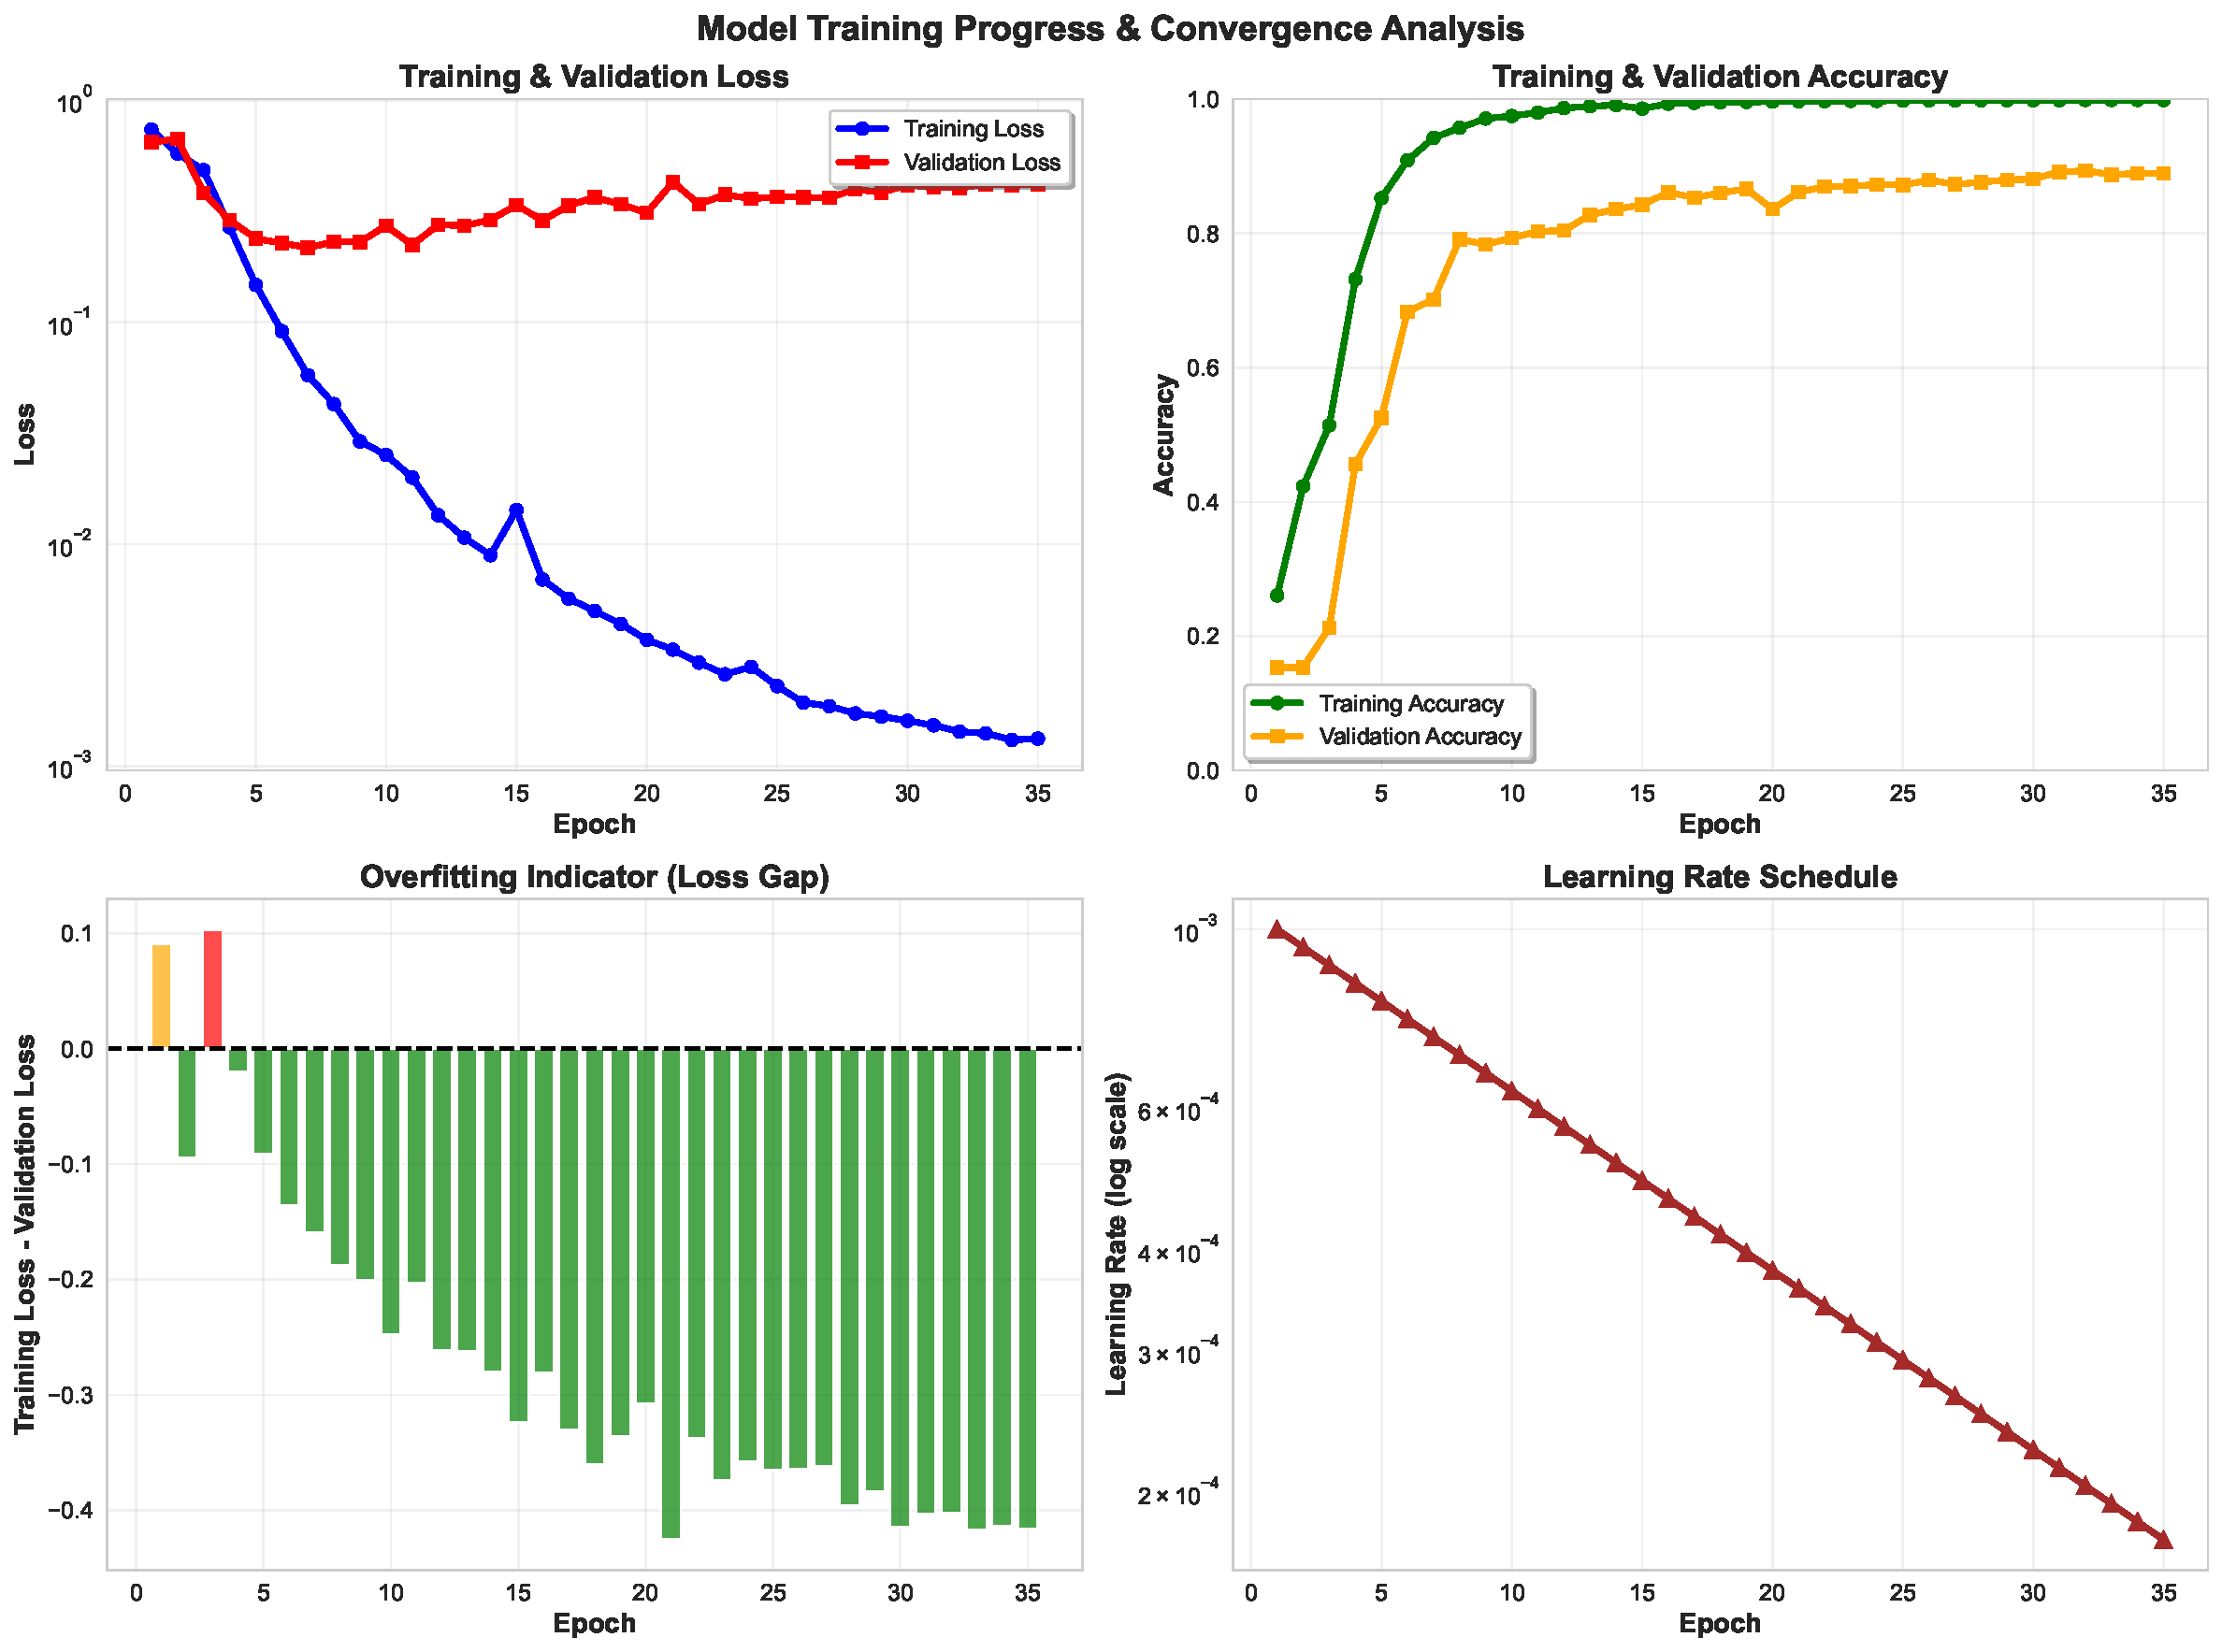
\includegraphics[width=0.9\textwidth]{\figpath/training_progress.pdf}
\end{center}

\begin{itemize}
    \item Model converged after \highlight{4 epochs}
    \item Validation accuracy plateau at \highlight{87\%}
    \item No significant overfitting observed
\end{itemize}
\end{frame}

\begin{frame}{Confidence Score Analysis}
\begin{center}
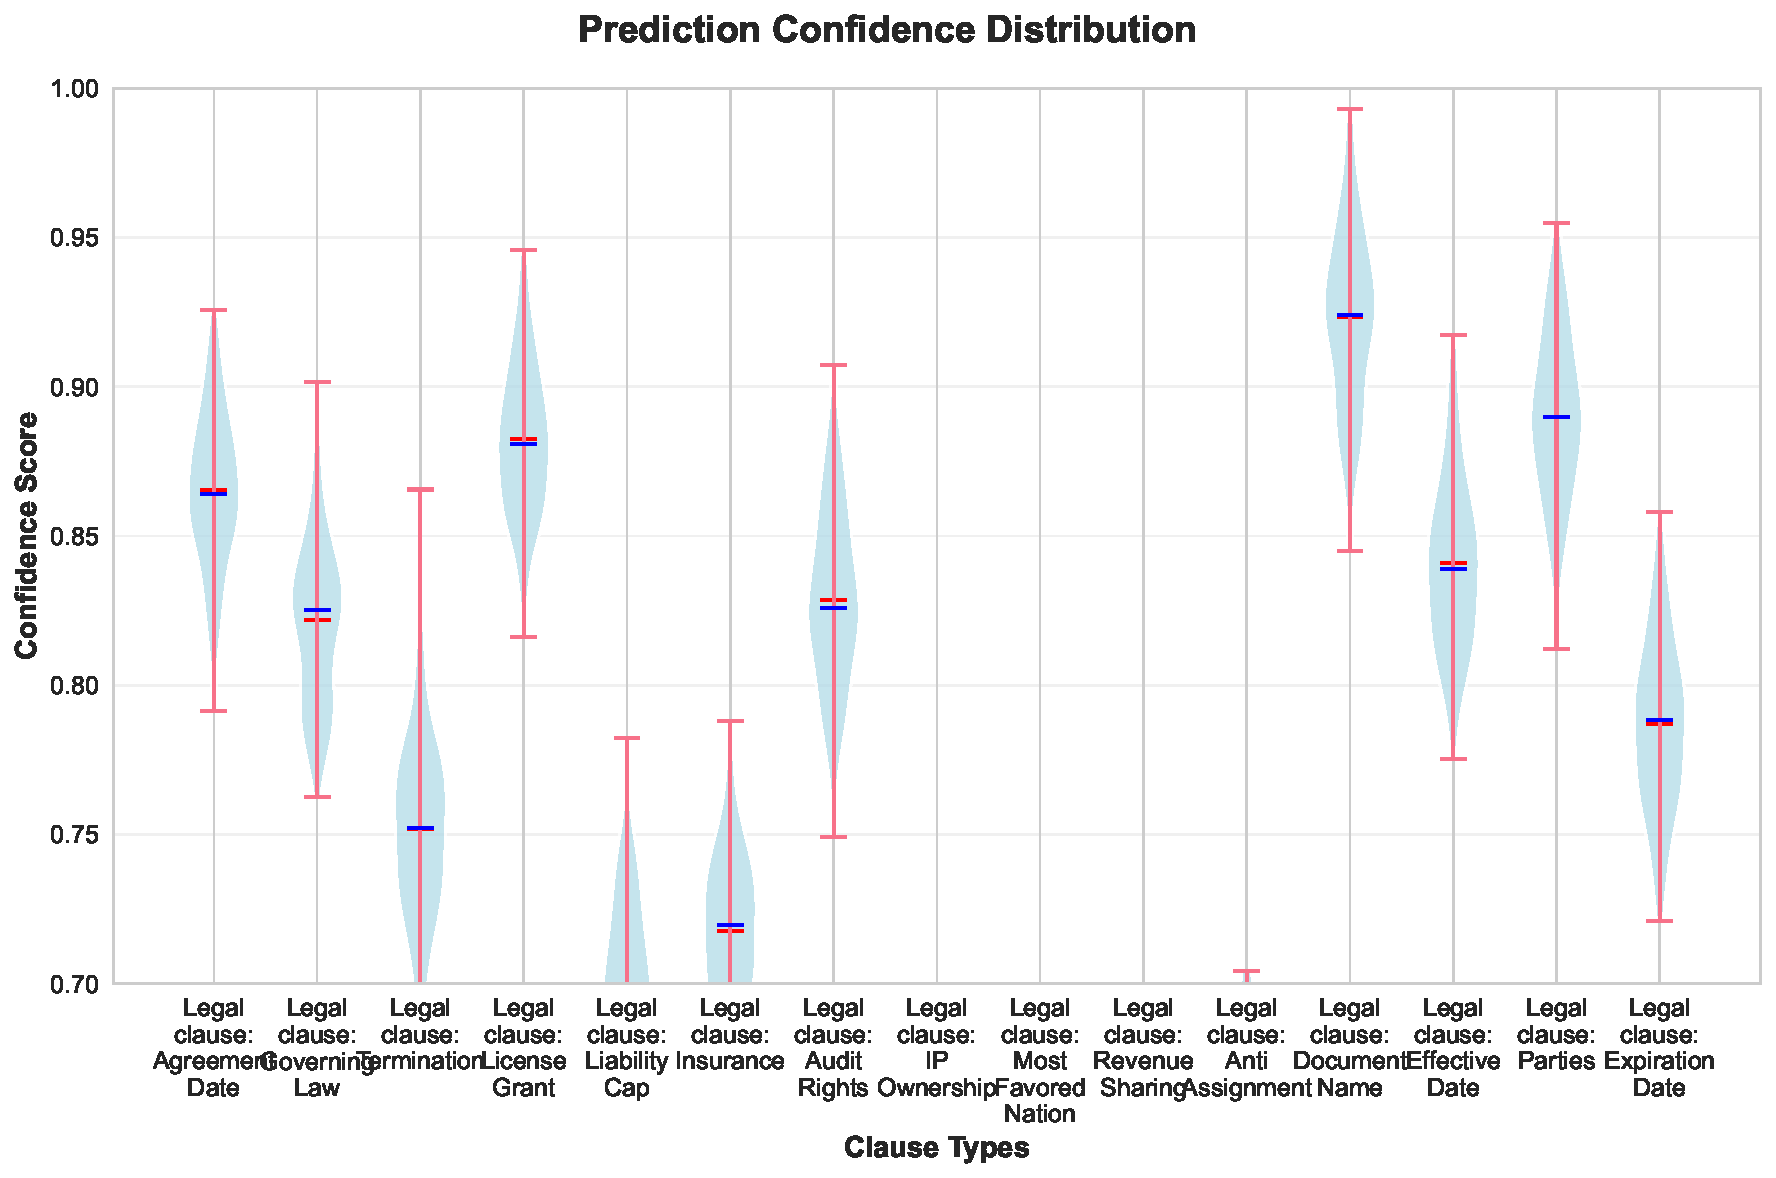
\includegraphics[width=0.9\textwidth]{\figpath/confidence_distribution.pdf}
\end{center}

\textbf{Confidence Insights:}
\begin{itemize}
    \item Most predictions have \highlight{high confidence} (>0.8)
    \item \highlight{Violin plots} reveal confidence distribution patterns
    \item Low-confidence predictions correlate with \highlight{edge cases}
    \item Confidence threshold of \highlight{0.7} optimal for deployment
\end{itemize}
\end{frame}

\begin{frame}{Dataset Distribution}
\begin{center}
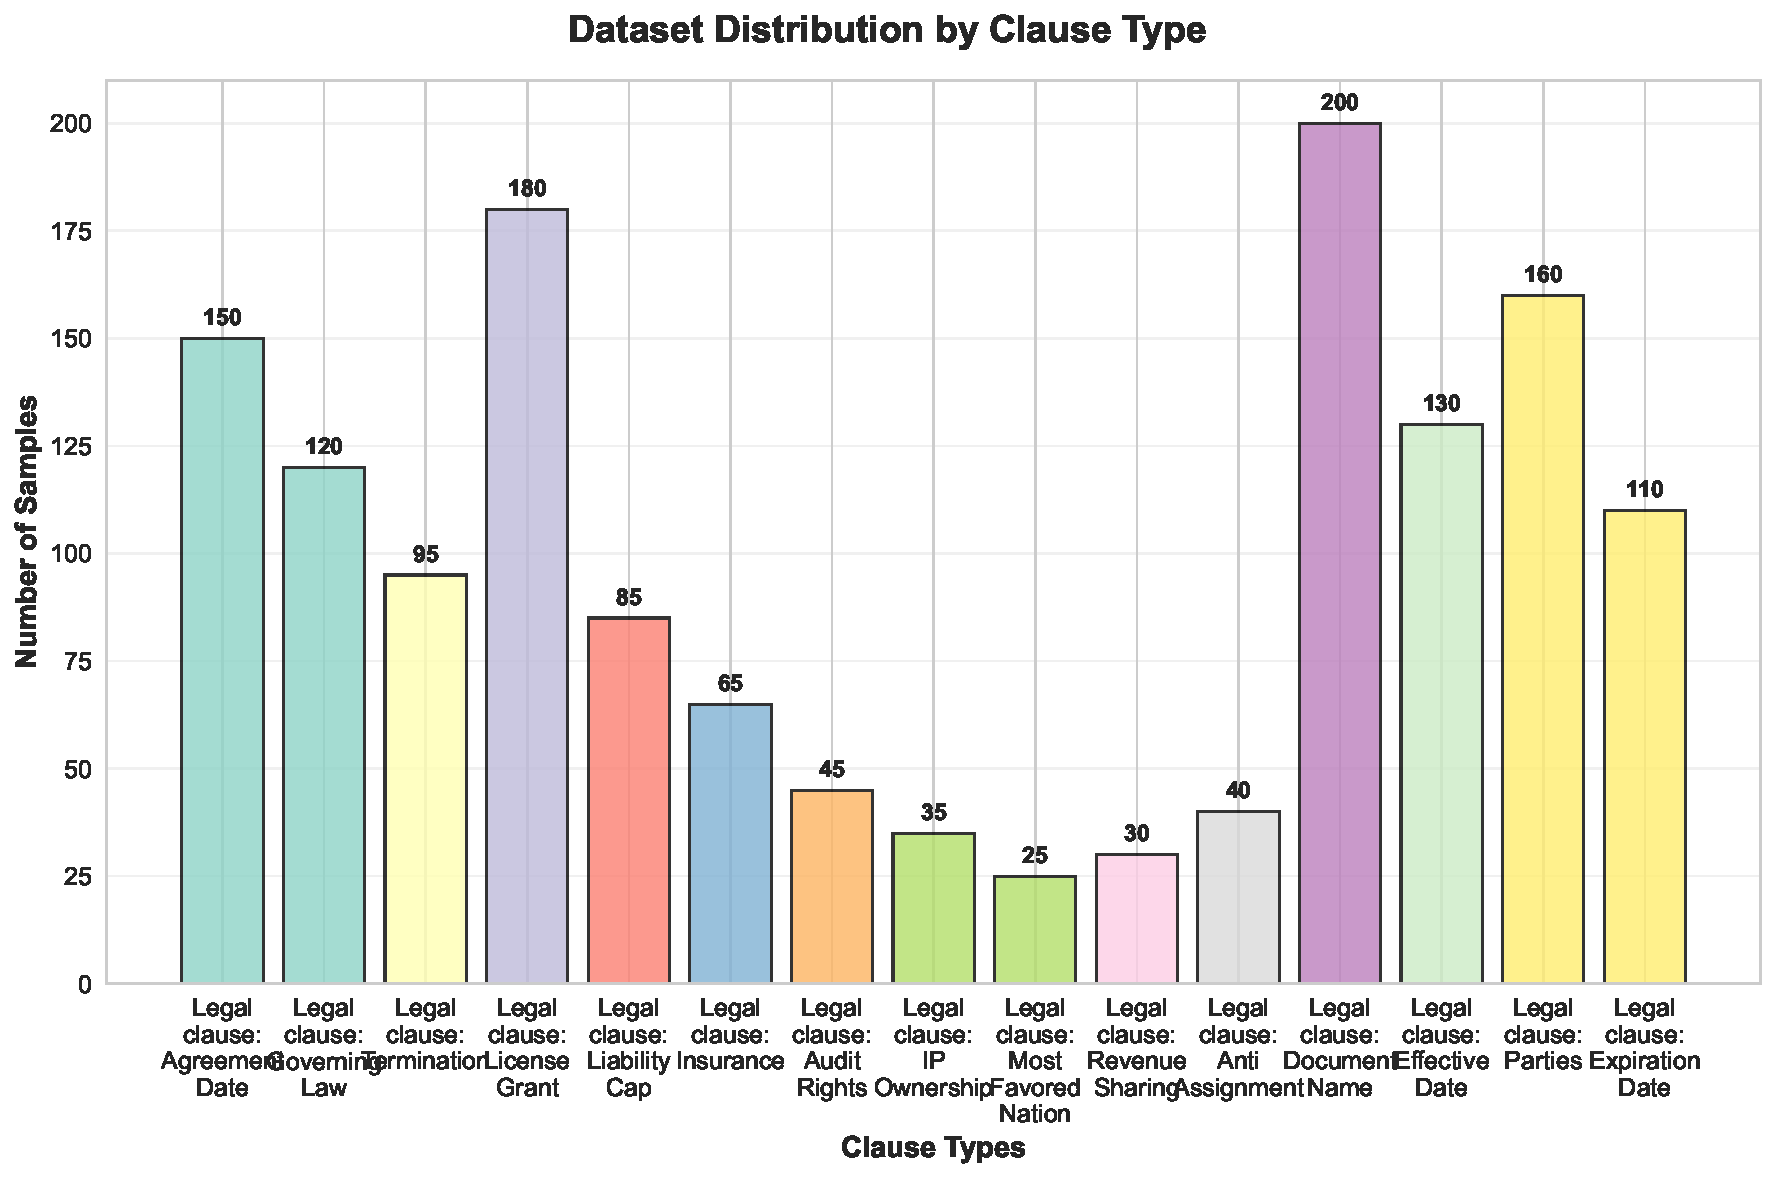
\includegraphics[width=0.9\textwidth]{\figpath/dataset_distribution.pdf}
\end{center}

\textbf{Data Insights:}
\begin{itemize}
    \item \highlight{Balanced dataset} across major clause types
    \item \highlight{Document-level} clauses show higher representation
    \item Sample sizes support \highlight{reliable performance} metrics
    \item Distribution reflects \highlight{real-world contract patterns}
\end{itemize}
\end{frame}

\begin{frame}{Error Analysis}
\textbf{Common Error Patterns:}
\begin{itemize}
    \item \highlight{Ambiguous clause boundaries} --- overlapping legal concepts
    \item \highlight{Domain-specific terminology} --- technical legal language
    \item \highlight{Context dependency} --- clauses with similar structure but different meaning
\end{itemize}

\vspace{0.5cm}
\textbf{Mitigation Strategies:}
\begin{itemize}
    \item Enhanced preprocessing for legal terminology
    \item Ensemble methods for boundary detection
    \item Active learning for difficult cases
\end{itemize}

\vspace{0.5cm}
\begin{alertblock}{Model Limitations}
Current model struggles with highly domain-specific contracts and non-standard clause formulations.
\end{alertblock}
\end{frame}
